% =====================================================================
%  Báo cáo môn Phân tích Dữ liệu — Trường Đại học Mở TP.HCM
%  Định dạng: NeurIPS-style (một cột, 10pt)
%
%  BIÊN DỊCH: XeLaTeX hoặc LuaLaTeX (KHÔNG dùng pdfLaTeX — cần font
%  hỗ trợ tiếng Việt). Trên Overleaf: Menu > Compiler > XeLaTeX.
%
%  Hình lấy từ ../analysis/figures/ — nếu nộp riêng file .tex thì copy
%  thư mục figures vào cùng chỗ và sửa \graphicspath bên dưới.
% =====================================================================
\documentclass[10pt]{article}

\usepackage{fontspec}
\setmainfont{Times New Roman}[Ligatures=TeX]
\usepackage{polyglossia}
\setmainlanguage{vietnamese}

\usepackage[a4paper, margin=1.9cm]{geometry}
\usepackage{booktabs}
\usepackage{graphicx}
\graphicspath{{../analysis/figures/}{figures/}}
\usepackage{caption}
\usepackage{subcaption}
\usepackage{float}
\usepackage{xcolor}
\usepackage{titlesec}
\usepackage[hidelinks]{hyperref}
\usepackage{enumitem}

\captionsetup{font=small, labelfont=bf, skip=3pt}
\setlist[itemize]{leftmargin=1.2em, itemsep=1pt, topsep=2pt}
\setlist[enumerate]{leftmargin=1.4em, itemsep=1pt, topsep=2pt}
\titleformat{\section}{\normalfont\large\bfseries}{\thesection}{0.6em}{}
\titleformat{\subsection}{\normalfont\normalsize\bfseries}{\thesubsection}{0.6em}{}
\titlespacing{\section}{0pt}{9pt}{4pt}
\titlespacing{\subsection}{0pt}{6pt}{3pt}
\setlength{\parskip}{3pt}
\setlength{\parindent}{0pt}
\renewcommand{\arraystretch}{1.06}

\newcommand{\keyfind}[1]{\textbf{#1}}

% ---------------------------------------------------------------------
\begin{document}

\begin{center}
{\LARGE\bfseries Phân tích thị trường việc làm ngành Dữ liệu tại Việt Nam}\\[4pt]
{\normalsize Bằng chứng từ 1.701 tin tuyển dụng trên sáu nền tảng}\\[12pt]

{\large Nguyễn Đức Bảo Hưng \textnormal{(2351060013)} \qquad Võ Trí Đạt \textnormal{(2351060008)}}\\[5pt]
{\normalsize Trường Đại học Mở Thành phố Hồ Chí Minh \quad\textbar\quad Môn học: Phân tích Dữ liệu}
\end{center}

\vspace{4pt}
\begin{center}
\begin{minipage}{0.93\textwidth}
{\bfseries Tóm tắt.}\; Người mới vào ngành dữ liệu ở Việt Nam nhận được rất nhiều lời khuyên nhưng
không có con số nào. Chúng tôi thu thập 1.701 tin tuyển dụng từ sáu nền tảng, gán nhãn nghề cho từng
tin bằng một quy trình ba tầng, và phân tích 720 tin thuộc ngành dữ liệu để trả lời ba câu hỏi:
thị trường \emph{đang tuyển gì}, \emph{vì sao lại như vậy}, và \emph{người học nên đi đường nào}.
Ba kết quả nổi bật đều đi ngược trực giác phổ biến: đây là thị trường \emph{phân tích} chứ không phải
thị trường \emph{xây mô hình}; Python \emph{không} phải thứ phân biệt một Data Analyst; và cửa vào
nghề hẹp không phải vì thiếu vị trí cho người mới mà vì tin tuyển người mới đòi hỏi gần bằng tin
tuyển người có kinh nghiệm.
\end{minipage}
\end{center}
\vspace{6pt}

% =====================================================================
\section{Giới thiệu và mục tiêu}

Thị trường tuyển dụng ngành dữ liệu ở Việt Nam \textbf{không thể đọc trực tiếp}, vì các nền tảng
tuyển dụng không có chuẩn tên nghề chung:

\begin{itemize}
\item \textbf{Tên nghề không thống nhất và song ngữ} --- \textit{Data Engineer}, \textit{Kỹ sư dữ liệu},
      \textit{Chuyên viên phân tích} có thể cùng chỉ một công việc.
\item \textbf{Nhiều nghề dữ liệu không nói ``data''} --- người làm BI mang chức danh
      \textit{Reporting Specialist}; kỹ sư ML mang chức danh \textit{AI Engineer}.
\item \textbf{Bẫy ngược lại} --- nhiều tin \emph{có} chữ \textit{Analyst} lại là công việc phần mềm hoặc
      ERP, không đụng tới dữ liệu.
\end{itemize}

Vì vậy trước khi trả lời bất kỳ câu hỏi thị trường nào, phải trả lời một câu trước:
\textbf{mỗi tin tuyển dụng thuộc nghề gì?}

\textbf{Mục tiêu của đề tài} là dựng một bộ dữ liệu tuyển dụng ngành dữ liệu \emph{đã được gán nhãn nghề
đáng tin cậy}, rồi từ đó trả lời ba nhóm câu hỏi theo mạch chuẩn của phân tích dữ liệu:

\begin{enumerate}
\item \textbf{Mô tả} --- thị trường đang tuyển những nghề gì, quy mô ra sao, cần kỹ năng nào?
\item \textbf{Chẩn đoán} --- vì sao thị trường lại có hình dạng đó?
\item \textbf{Đề xuất} --- người học nên học gì và đi theo lộ trình nào?
\end{enumerate}

\subsection{Quy trình xử lý}

\begin{center}
\small
\fbox{\parbox{0.94\textwidth}{\centering
6 nền tảng tuyển dụng $\rightarrow$ \textbf{Thô} (tin nguyên bản) $\rightarrow$ \textbf{Kho dữ liệu}
(DuckDB) $\rightarrow$ \textbf{Chuẩn hoá} (kỹ năng / cấp bậc / địa điểm / doanh nghiệp + khử trùng lặp)
$\rightarrow$ \textbf{Gán nhãn nghề} $\rightarrow$ \textbf{Bảng tổng hợp} $\rightarrow$ Phân tích
}}
\end{center}

Mỗi tầng làm đúng một việc. Tầng \emph{Bảng tổng hợp} tồn tại để mọi phân tích dùng chung một định nghĩa
``tập phân tích'', tránh tình trạng hai bảng số lại dựa trên hai mẫu số khác nhau.

% =====================================================================
\section{Dữ liệu}

\begin{center}
\small
\begin{tabular}{lrr}
\toprule
\textbf{Bảng} & \textbf{Số dòng} & \textbf{Số thuộc tính} \\
\midrule
Tin thô thu thập được          & 1.701 & 20 \\
Sau chuẩn hoá (\textit{jobs\_silver}) & 1.701 & 30 \\
\textbf{Tập phân tích}         & \textbf{720} & 30 \\
\bottomrule
\end{tabular}
\end{center}

Dữ liệu thu thập tại \textbf{một lát cắt thời gian ngày 16/06/2026} từ VietnamWorks, CareerViet, ITviec,
TopCV, TopDev và Glints. Tập phân tích 720 tin có được sau khi loại \textbf{882 tin} không thuộc ngành
dữ liệu và \textbf{147 tin} trùng lặp chéo nguồn.

Các thuộc tính chính sau chuẩn hoá: tên nghề, nhánh nghề, cấp bậc, danh sách kỹ năng đã chuẩn hoá,
số lượng kỹ năng, thành phố, ngành của doanh nghiệp, hình thức làm việc (tại chỗ / từ xa), ngày đăng,
và các cột ghi lại \emph{nguồn gốc} của từng giá trị suy luận.

% =====================================================================
\section{Phương pháp}

\subsection{Gán nhãn nghề bằng quy trình ba tầng}

Nhãn nghề là đầu vào của mọi con số phía sau, nên phần lớn công sức kỹ thuật nằm ở đây. Chúng tôi dùng
một quy trình \emph{rẻ và hẹp trước, đắt sau}:

\begin{enumerate}
\item \textbf{Quy tắc trên tiêu đề} --- khớp danh sách bí danh hẹp do người soạn, không đọc mô tả công
      việc. Quyết định 426/720 tin.
\item \textbf{So khớp ngữ nghĩa} --- so sánh tin với vector mẫu của từng nghề, chỉ nhận khi một nghề
      thắng rõ rệt. Sau khi siết ngưỡng, tầng này gần như không nhận tin nào --- tin mơ hồ phải rơi
      xuống tầng biết đọc mô tả.
\item \textbf{Nhiều mô hình ngôn ngữ bỏ phiếu} --- mỗi tin cần \textbf{ít nhất hai mô hình độc lập đồng
      thuận}; bất đồng thì mô hình thứ ba phân xử. Vẫn không ngã ngũ thì thu hẹp danh sách lựa chọn về
      đúng các nghề đang tranh chấp và cho đọc toàn văn mô tả.
\end{enumerate}

Kết quả là 20 nghề, gộp thành 5 nhánh. Mỗi tin ghi lại \emph{tầng nào đã quyết định nhãn}.

\subsection{Kiểm định chất lượng nhãn}

Chúng tôi lấy mẫu phân tầng 30 tin và \textbf{gán nhãn mù}: người gán ẩn hoàn toàn đáp án của hệ thống,
quyết định xong mới đối chiếu. Kết quả \textbf{29/30 = 96,7\%} (khoảng tin cậy 95\%: 83,3--99,4\%).
Tách theo tầng: tầng mô hình ngôn ngữ đúng 18/18 và 3/3, tầng quy tắc tiêu đề 8/9. Trường \emph{cấp bậc}
cũng được kiểm định mù bằng hai giám định độc lập: 86,2\% đúng bậc.

\subsection{Các phép phân tích}

Toàn bộ phân tích dựa trên \emph{đếm và so sánh tập hợp}, không dùng mô hình dự đoán --- dữ liệu không có
trường lương nên không tồn tại biến mục tiêu để dự đoán. Ba phép chính:

\begin{itemize}
\item \textbf{Thị phần} --- đếm số tin theo nghề, nhánh, cấp bậc, ngành doanh nghiệp.
\item \textbf{Lift kỹ năng} --- tỉ lệ một kỹ năng trong một nghề chia cho tỉ lệ của nó trên toàn thị
      trường. Lift $>1$ nghĩa là kỹ năng đó \emph{đặc trưng} cho nghề, $\approx 1$ nghĩa là nó phổ biến
      khắp nơi và \emph{không phân biệt} được gì.
\item \textbf{Ma trận chuyển nghề} --- mỗi nghề có một \emph{hồ sơ kỹ năng} (các kỹ năng xuất hiện ở
      $\geq$25\% số tin của nghề đó). Ô $(A \rightarrow B)$ = phần trăm hồ sơ của $B$ mà người làm $A$
      đã có sẵn, tức $|hs(A) \cap hs(B)| / |hs(B)|$. Phép này bất đối xứng, và chính sự bất đối xứng
      là phát hiện.
\end{itemize}

% =====================================================================
\section{Kết quả 1 --- Mô tả: thị trường trông ra sao}

\begin{figure}[H]
\centering
\begin{subfigure}{0.49\textwidth}
  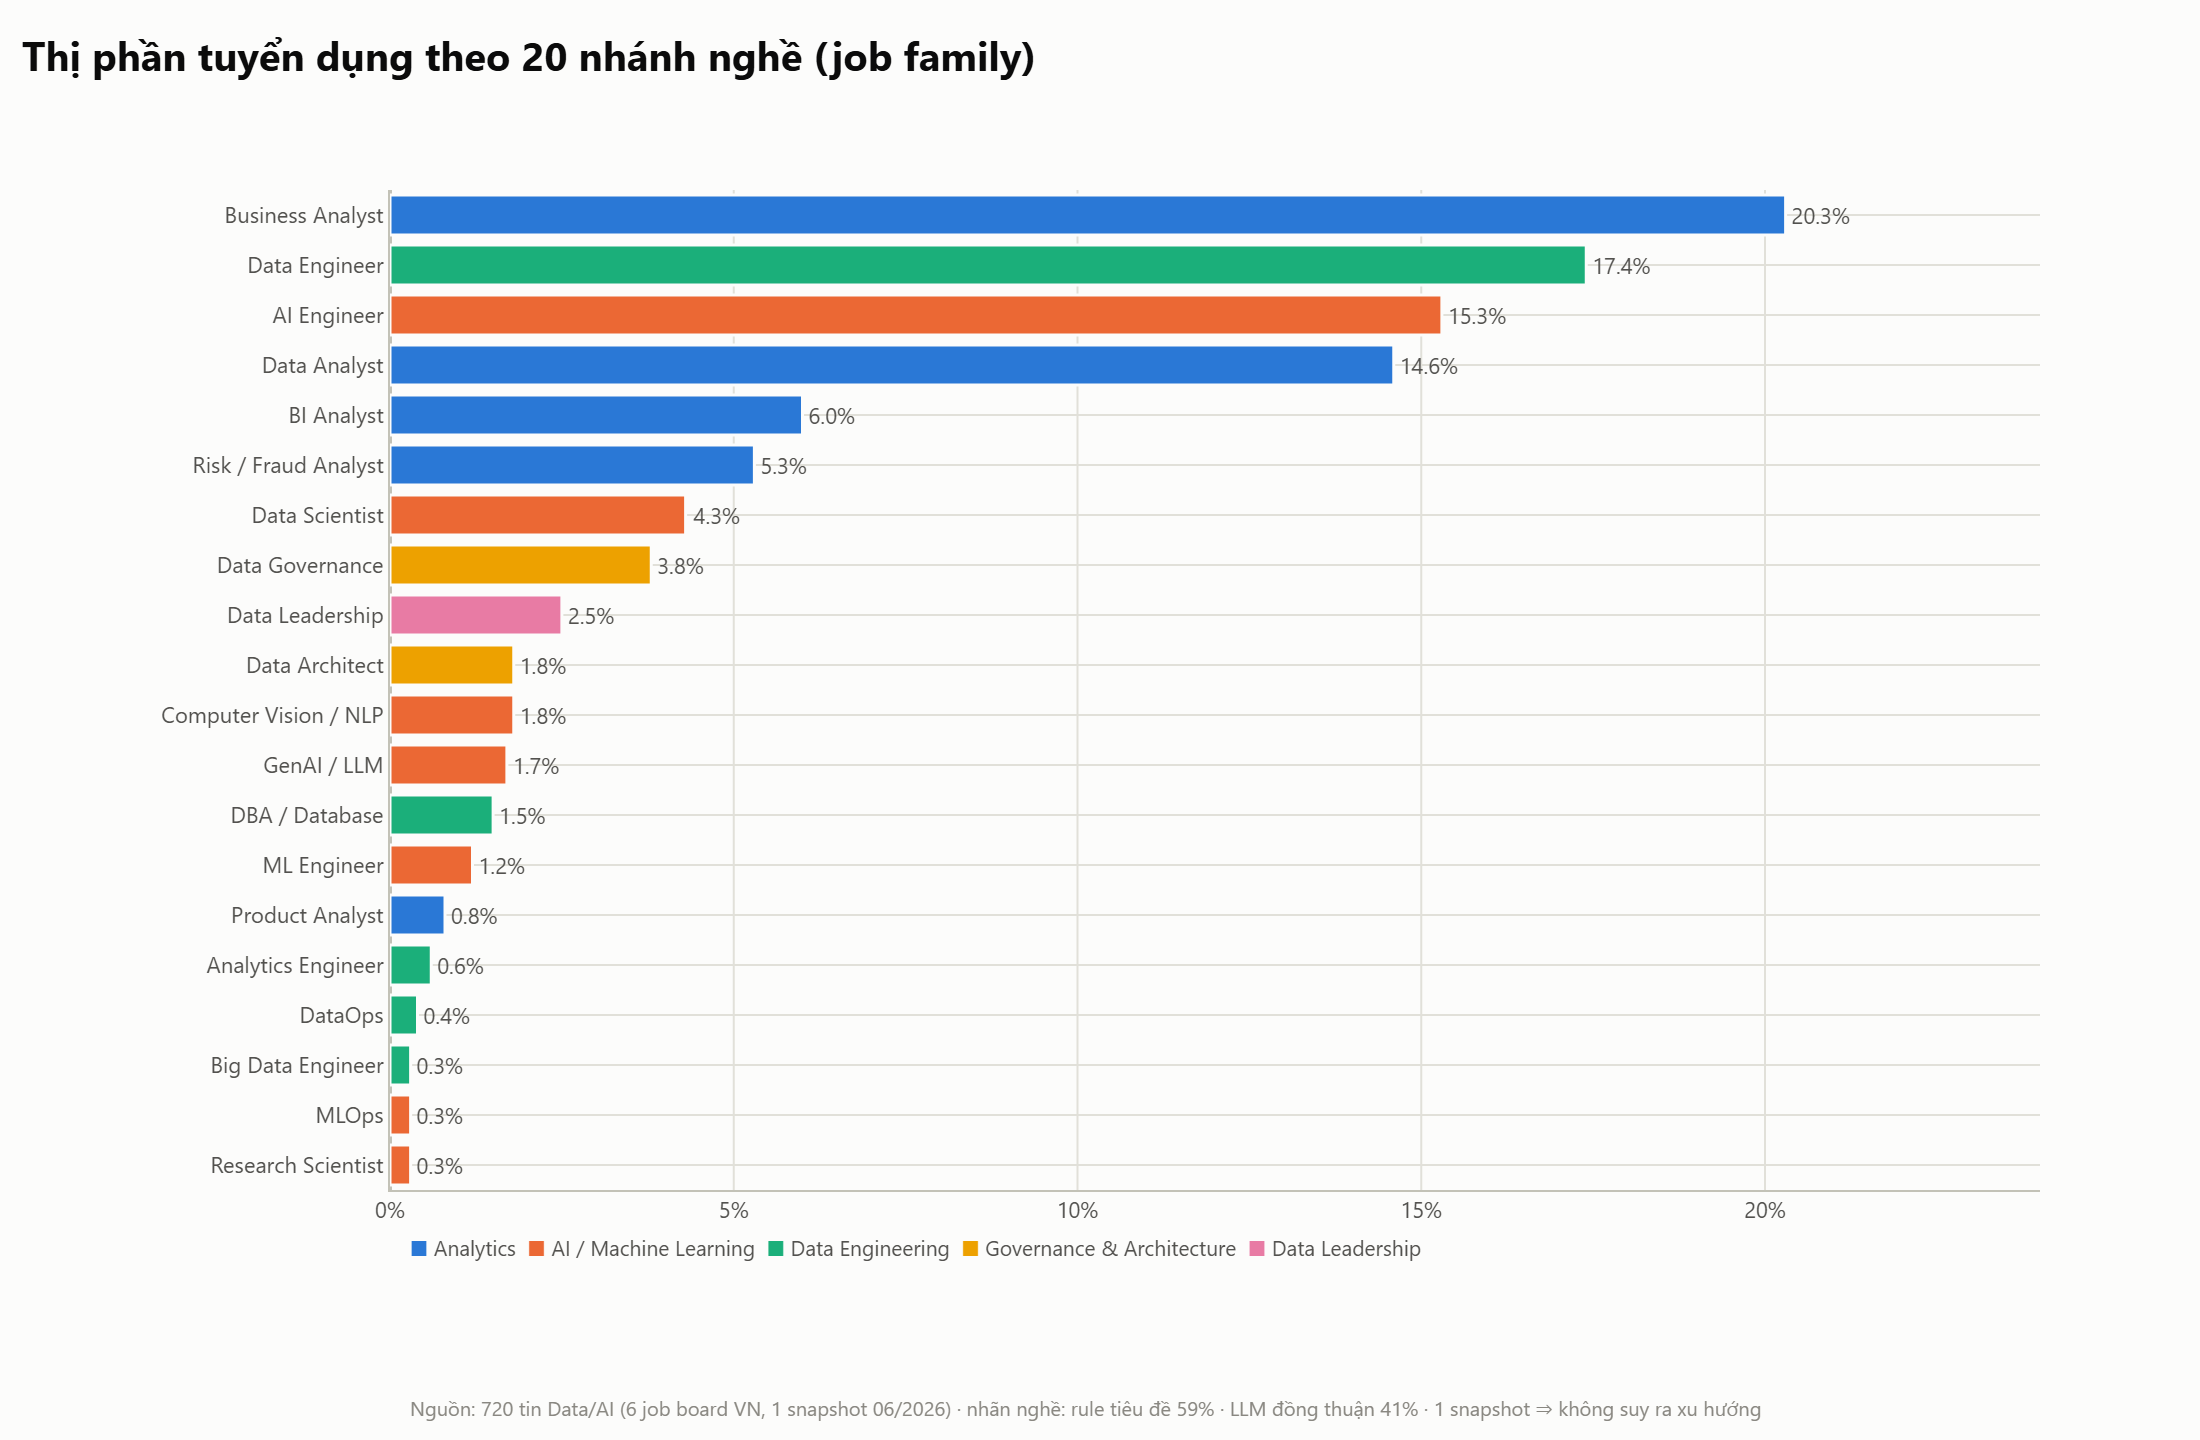
\includegraphics[width=\linewidth]{family_share.png}
  \caption{Thị phần theo nghề}
\end{subfigure}\hfill
\begin{subfigure}{0.49\textwidth}
  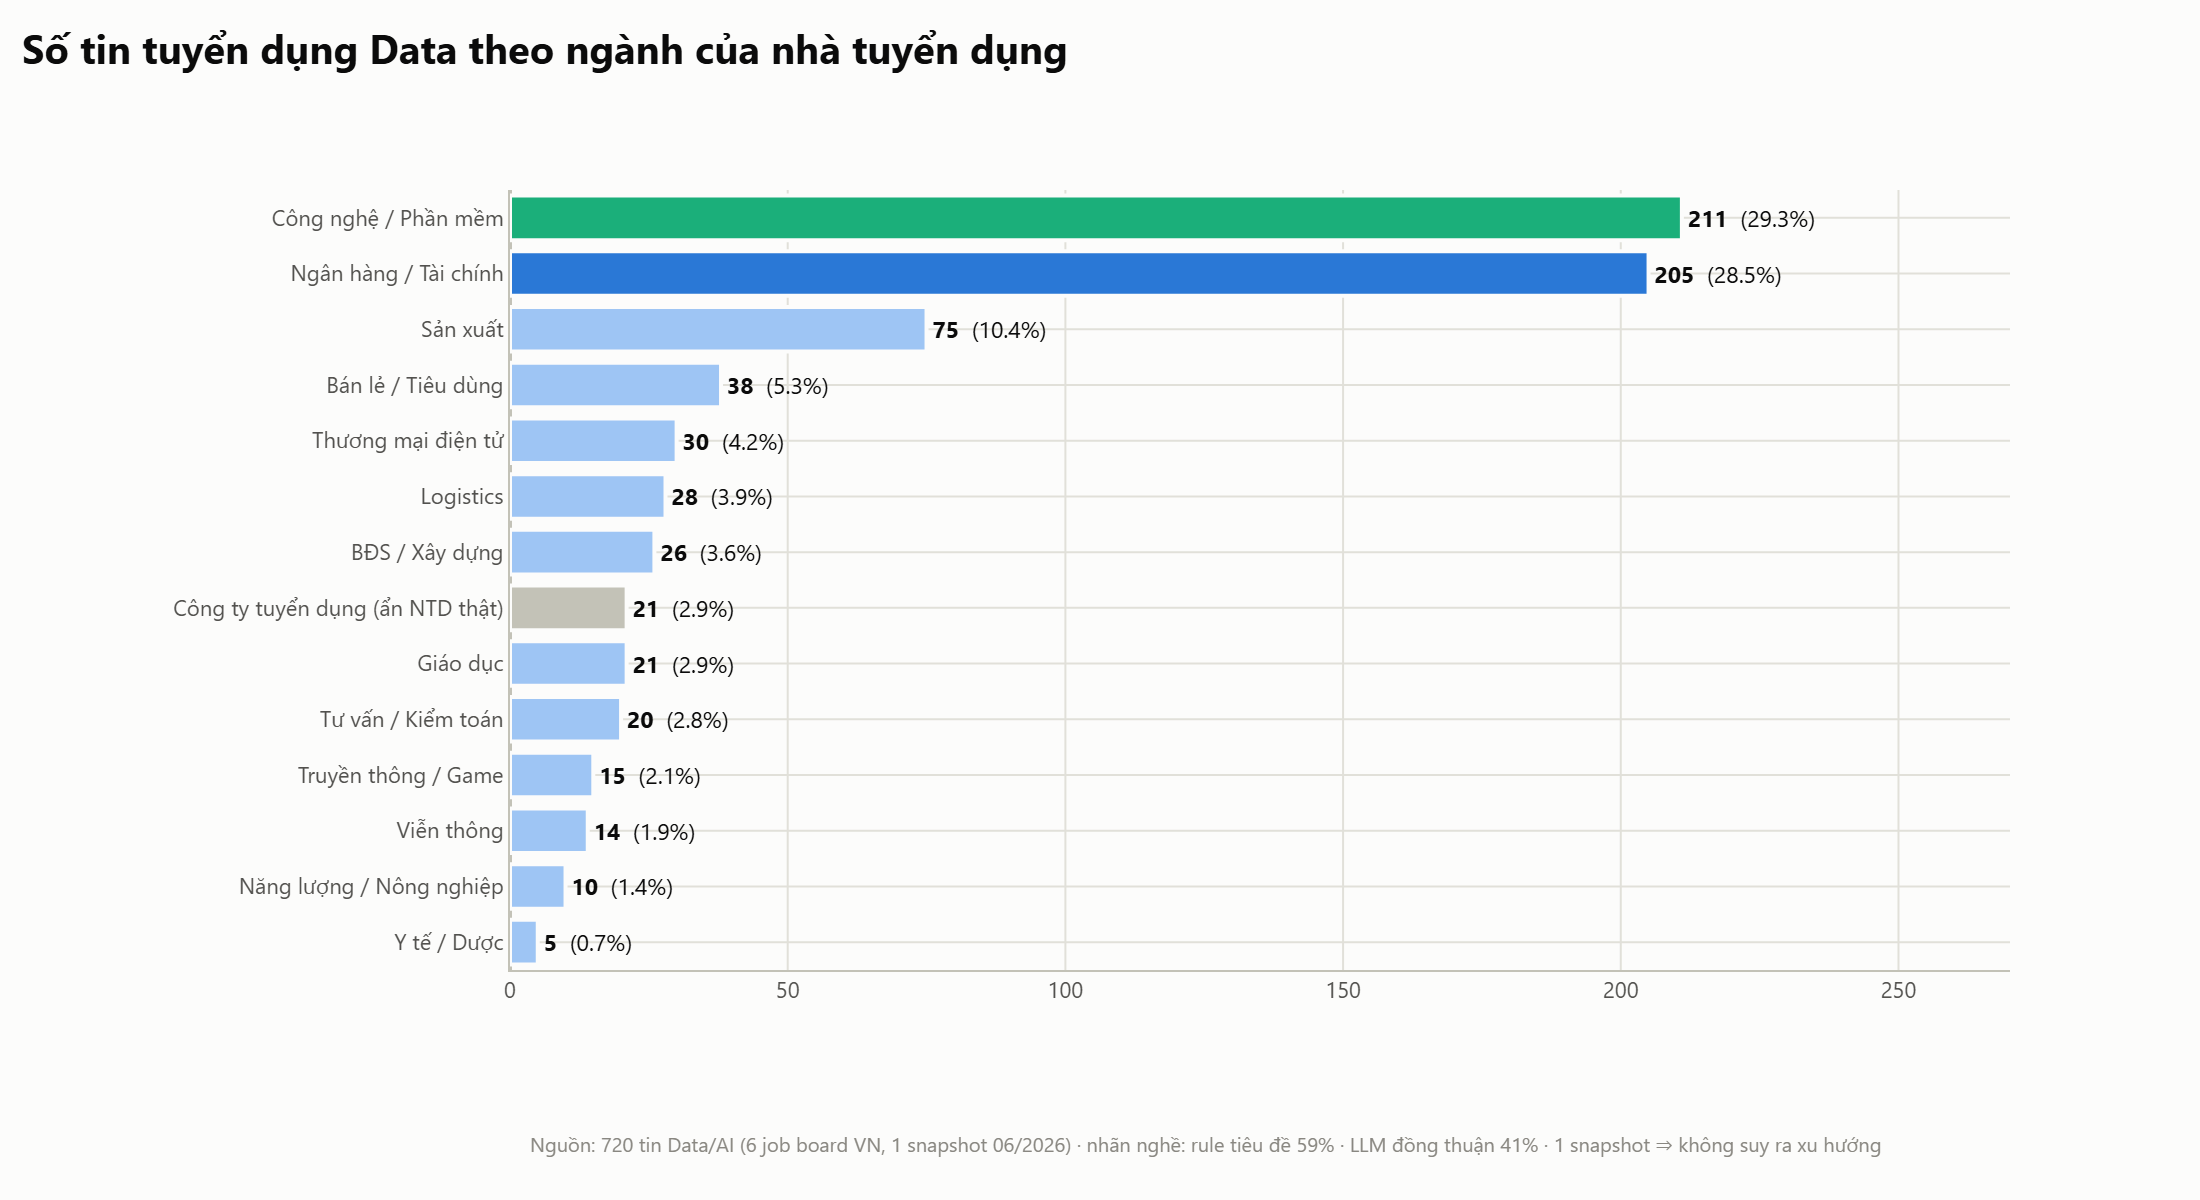
\includegraphics[width=\linewidth]{industry_share.png}
  \caption{Ngành của nhà tuyển dụng}
\end{subfigure}
\caption{Cấu trúc thị trường trên 720 tin tuyển dụng ngành dữ liệu.}
\end{figure}

\subsection{Không có ``nghề hot nhất'' --- có bốn cửa vào rộng gần bằng nhau}

Business Analyst 146 tin \textbar\ Data Engineer 125 \textbar\ AI Engineer 110 \textbar\ Data Analyst 105.
Bốn nghề này cộng lại chiếm \textbf{gần 2/3 thị trường}, và chênh lệch giữa chúng \emph{nhỏ hơn sai số của
phép đo} (với 720 tin, sai số của một tỉ lệ khoảng 15--20\% là $\pm$3 điểm phần trăm).

\keyfind{Vì vậy chúng tôi cố ý không xếp hạng bốn nghề này.} Cách đọc đúng là ``bốn cửa vào rộng gần
bằng nhau'', không phải ``nghề X đang dẫn đầu''.

Ở cấp nhánh thì khoảng cách đủ lớn để nói: Analytics \textbf{46,9\%}, AI/Machine Learning 24,9\%,
Data Engineering 20,1\%. Trong khi đó các vai trò xây mô hình thuần rất mỏng --- \keyfind{Data Scientist
chỉ 4,3\%}. Truyền thông nói nhiều về AI, nhưng thị trường tuyển nhiều nhất là người đọc số và làm báo cáo.

\subsection{Ai đang tuyển: công nghệ và ngân hàng, ngang nhau}

Công nghệ/Phần mềm \textbf{211 tin (29,3\%)} và Ngân hàng/Tài chính \textbf{205 tin (28,5\%)} --- chênh
0,8 điểm phần trăm, coi như bằng nhau. Kế đến là Sản xuất 75 tin (10,4\%). Hai khối dẫn đầu cộng lại
chiếm gần 58\% thị trường.

\subsection{Bộ kỹ năng lõi của ngành: SQL, Python, phân tích dữ liệu}

SQL \textbf{47,8\%} \textbar\ Python \textbf{43,5\%} \textbar\ Data Analysis \textbf{39,6\%} \textbar\
Reporting 38,3\%.

Đây là \emph{lõi chung} chạy xuyên mọi nghề: học ba thứ này thì mở được cửa ở mọi nhánh. Điều đáng chú ý
là sự khác biệt giữa các nghề \textbf{không nằm ở lõi} --- sẽ quay lại ở Mục 5.

\subsection{Tiếng Anh là kỹ năng thật, không phải điểm cộng}

\textbf{33,8\%} tin yêu cầu tiếng Anh --- đứng thứ năm, trên cả Machine Learning. Và nó lệch rất mạnh
theo ngành: công ty công nghệ \textbf{48,8\%}, logistics 32,1\%, ngân hàng 25,4\%, thương mại điện tử chỉ
\textbf{16,7\%}. Vào công ty công nghệ thì cứ hai tin có một tin đòi tiếng Anh; vào thương mại điện tử
thì sáu tin mới có một.

\subsection{Hai kết quả âm tính, vẫn đáng báo cáo}

\keyfind{Làm việc từ xa gần như không tồn tại:} chỉ \textbf{35/720 tin (4,9\%)}.

\keyfind{Thị trường tập trung tuyệt đối ở hai thành phố:} Hà Nội 325 tin, TP.HCM 303 tin, và
\textbf{toàn bộ các tỉnh/thành còn lại cộng lại chỉ 25 tin}. Hơn nữa \emph{cơ cấu nghề ở hai thành phố
gần như giống hệt nhau} (Analytics 45,5\% so với 49,8\%) --- chuyển thành phố không đổi được \emph{loại}
công việc làm được, chỉ đổi \emph{số lượng} tin.

% =====================================================================
\section{Kết quả 2 --- Chẩn đoán: vì sao thị trường lại như vậy}

\begin{figure}[H]
\centering
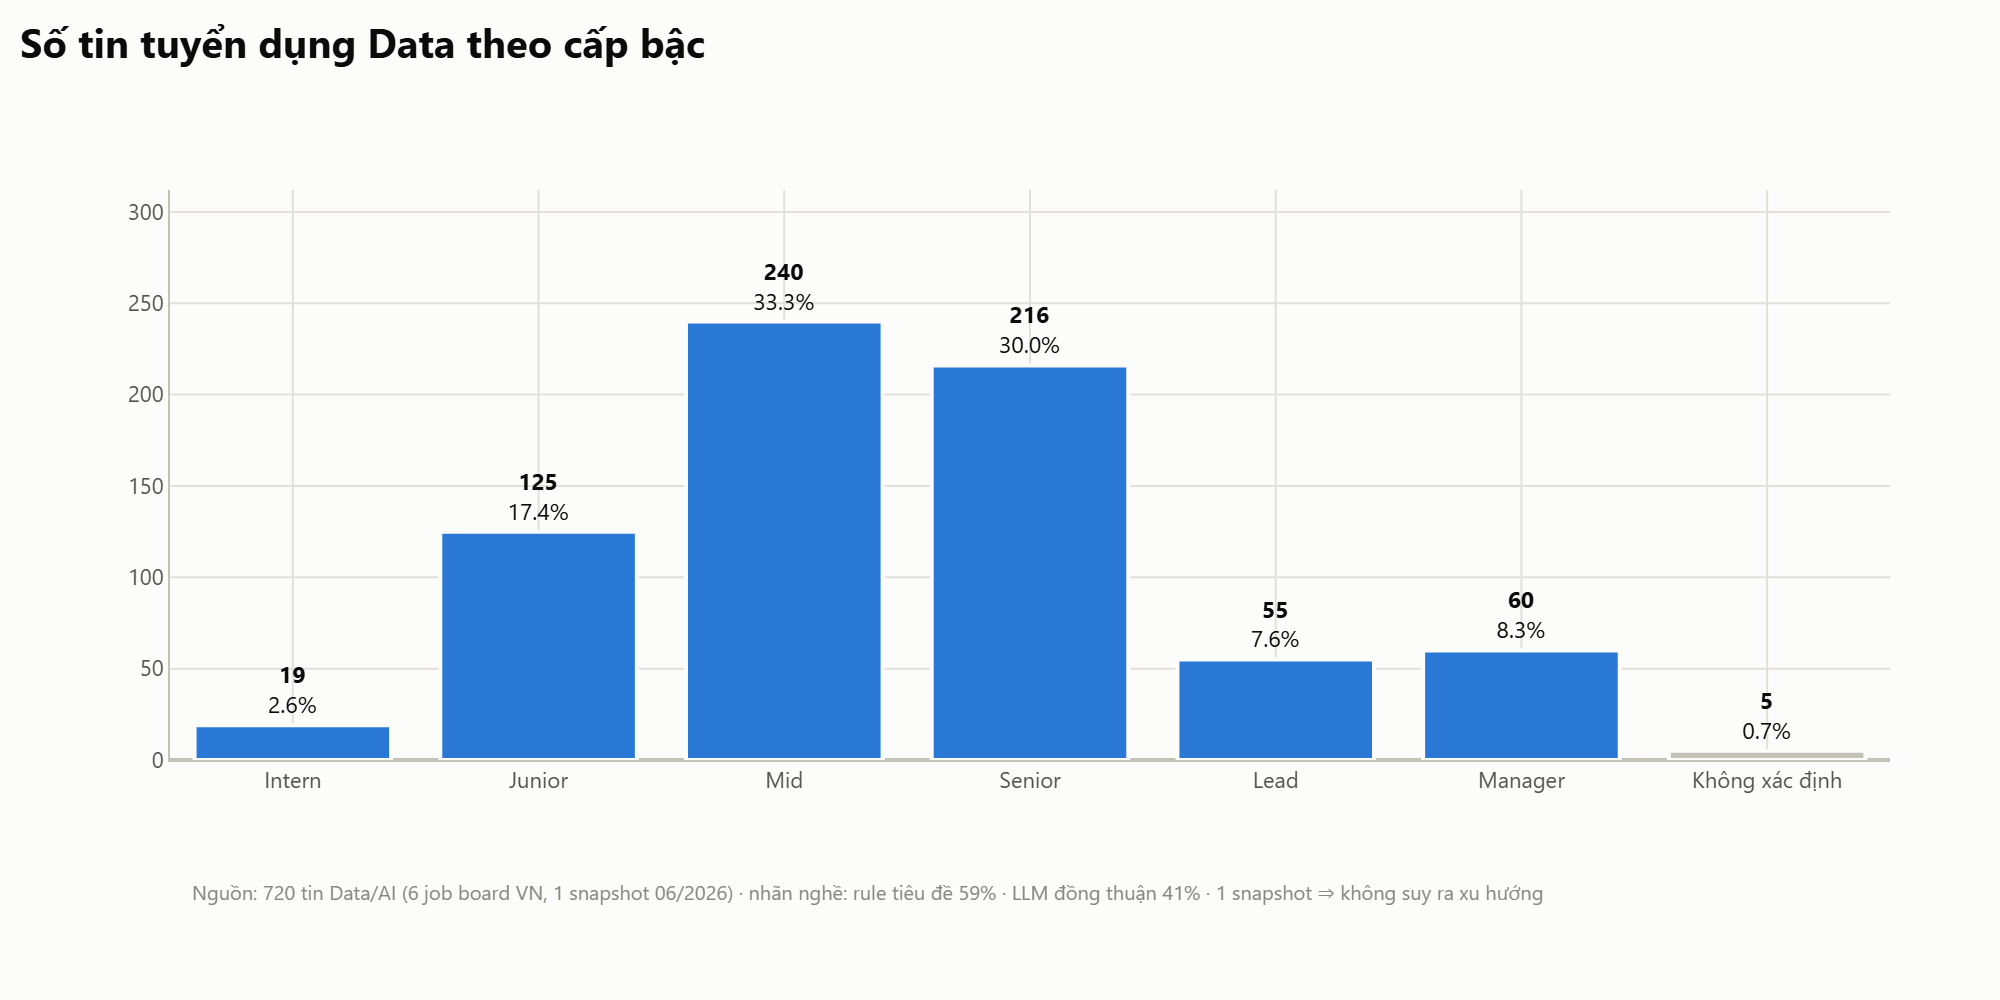
\includegraphics[width=0.72\textwidth]{seniority_share.png}
\caption{Phân bố cấp bậc. Mid và Senior chiếm 63\% thị trường.}
\end{figure}

\subsection{Cửa vào hẹp --- nhưng không phải vì thiếu vị trí cho người mới}

Junior 17,4\% và Intern 2,6\%, cộng lại \textbf{20\%}. Trong khi Mid 33,3\% và Senior 30,0\% chiếm tới
\textbf{63\%}. Thị trường rõ ràng ưu tiên người đã có kinh nghiệm.

Một cách giải thích hợp lý nằm ở \emph{đặc thù phát triển của ngành}: nhu cầu dữ liệu ở Việt Nam phần
lớn đến \emph{sau} khi doanh nghiệp đã vận hành ổn định và muốn khai thác dữ liệu sẵn có. Bộ phận dữ liệu
thường được lập ra để giải quyết một bài toán đã tồn tại, nên doanh nghiệp cần người làm được ngay hơn là
người cần đào tạo. Cần nói rõ đây là \emph{diễn giải}, dữ liệu trong đề tài không kiểm chứng được nó.

Nhưng dữ liệu \emph{có} nói được một điều cụ thể hơn, và nó bất ngờ:

\begin{center}
\small
\begin{tabular}{lrr}
\toprule
\textbf{Cấp bậc} & \textbf{Số tin} & \textbf{Số kỹ năng trung bình} \\
\midrule
Intern & 19  & 8,3 \\
Junior & 125 & \textbf{8,2} \\
Mid    & 240 & \textbf{9,8} \\
Senior & 216 & 9,9 \\
\bottomrule
\end{tabular}
\end{center}

\keyfind{Tin Junior đòi 8,2 kỹ năng, tin Mid đòi 9,8 --- chênh chưa tới hai kỹ năng.} Nếu khoảng cách
giữa hai cấp bậc chỉ là \emph{hai kỹ năng}, thì rào cản thật sự không nằm ở \emph{số lượng kỹ năng} mà
nằm ở \textbf{kinh nghiệm thực chiến} --- thứ mà tin tuyển dụng không liệt kê thành kỹ năng được.

Điều này đổi hẳn hàm ý cho người học: học thêm công cụ thứ mười không giúp bạn vượt rào; làm được một
việc thật mới giúp.

\subsection{Công nghệ và ngân hàng tuyển ngang nhau, nhưng tuyển hai thứ khác nhau}

\begin{center}
\small
\begin{tabular}{lrr}
\toprule
\textbf{Nghề} & \textbf{Công nghệ/Phần mềm} & \textbf{Ngân hàng/Tài chính} \\
\midrule
AI Engineer       & \textbf{53} & 19 \\
Business Analyst  & 43 & 38 \\
Data Engineer     & 47 & 37 \\
Risk / Fraud      & $\sim$0 & \textbf{29} \\
Data Governance   & 4  & \textbf{14} \\
\bottomrule
\end{tabular}
\end{center}

Công ty công nghệ tuyển AI Engineer \emph{gần gấp ba} ngân hàng. Ngược lại, ngân hàng gần như độc chiếm
hai nhánh: \keyfind{Risk/Fraud 29 trong tổng 38 tin} và \keyfind{Data Governance 14 trong tổng 27 tin}
của toàn thị trường --- hai nhánh sinh ra từ \emph{áp lực tuân thủ pháp lý} chứ không từ nhu cầu tự nhiên.

Hai khối tuyển số lượng như nhau nhưng gần như \textbf{không cạnh tranh nhau} về nhân sự.

\subsection{Python không phải thứ làm nên một Data Analyst}

Python xuất hiện ở 42,9\% tin Data Analyst --- nghe như yêu cầu quan trọng. Nhưng nó cũng xuất hiện ở
\textbf{43,5\% toàn thị trường}, tức \keyfind{lift $= 0{,}99$ --- không phân biệt được gì}.

\begin{center}
\small
\begin{tabular}{lrrr}
\toprule
\textbf{Kỹ năng} & \textbf{Trong Data Analyst} & \textbf{Toàn thị trường} & \textbf{Lift} \\
\midrule
Tableau    & 38,1\% & 12,8\% & \textbf{2,98} \\
Excel      & 37,1\% & 14,6\% & \textbf{2,54} \\
Power BI   & 61,9\% & 24,4\% & \textbf{2,53} \\
Statistics & 41,0\% & 16,3\% & \textbf{2,52} \\
\textbf{Python} & \textbf{42,9\%} & \textbf{43,5\%} & \textbf{0,99} \\
\bottomrule
\end{tabular}
\end{center}

Lời khuyên phổ biến ``muốn làm Data Analyst thì học Python'' không sai, nhưng nó chỉ đưa người học tới
\emph{mức trung bình} của thị trường. Thứ \emph{phân biệt} là công cụ trực quan hoá.

Tương tự với AI Engineer: nghề này dùng SQL chỉ \textbf{25,5\%} --- \emph{thấp hơn} mặt bằng 47,8\% ---
nhưng API 56,4\% và Docker 33,6\%. \keyfind{``AI Engineer'' trong tin tuyển dụng Việt Nam là kỹ sư phần
mềm biết đưa mô hình lên chạy thật, không phải nhà toán học.}

% =====================================================================
\section{Kết quả 3 --- Đề xuất: nên học gì và đi đường nào}

\begin{figure}[H]
\centering
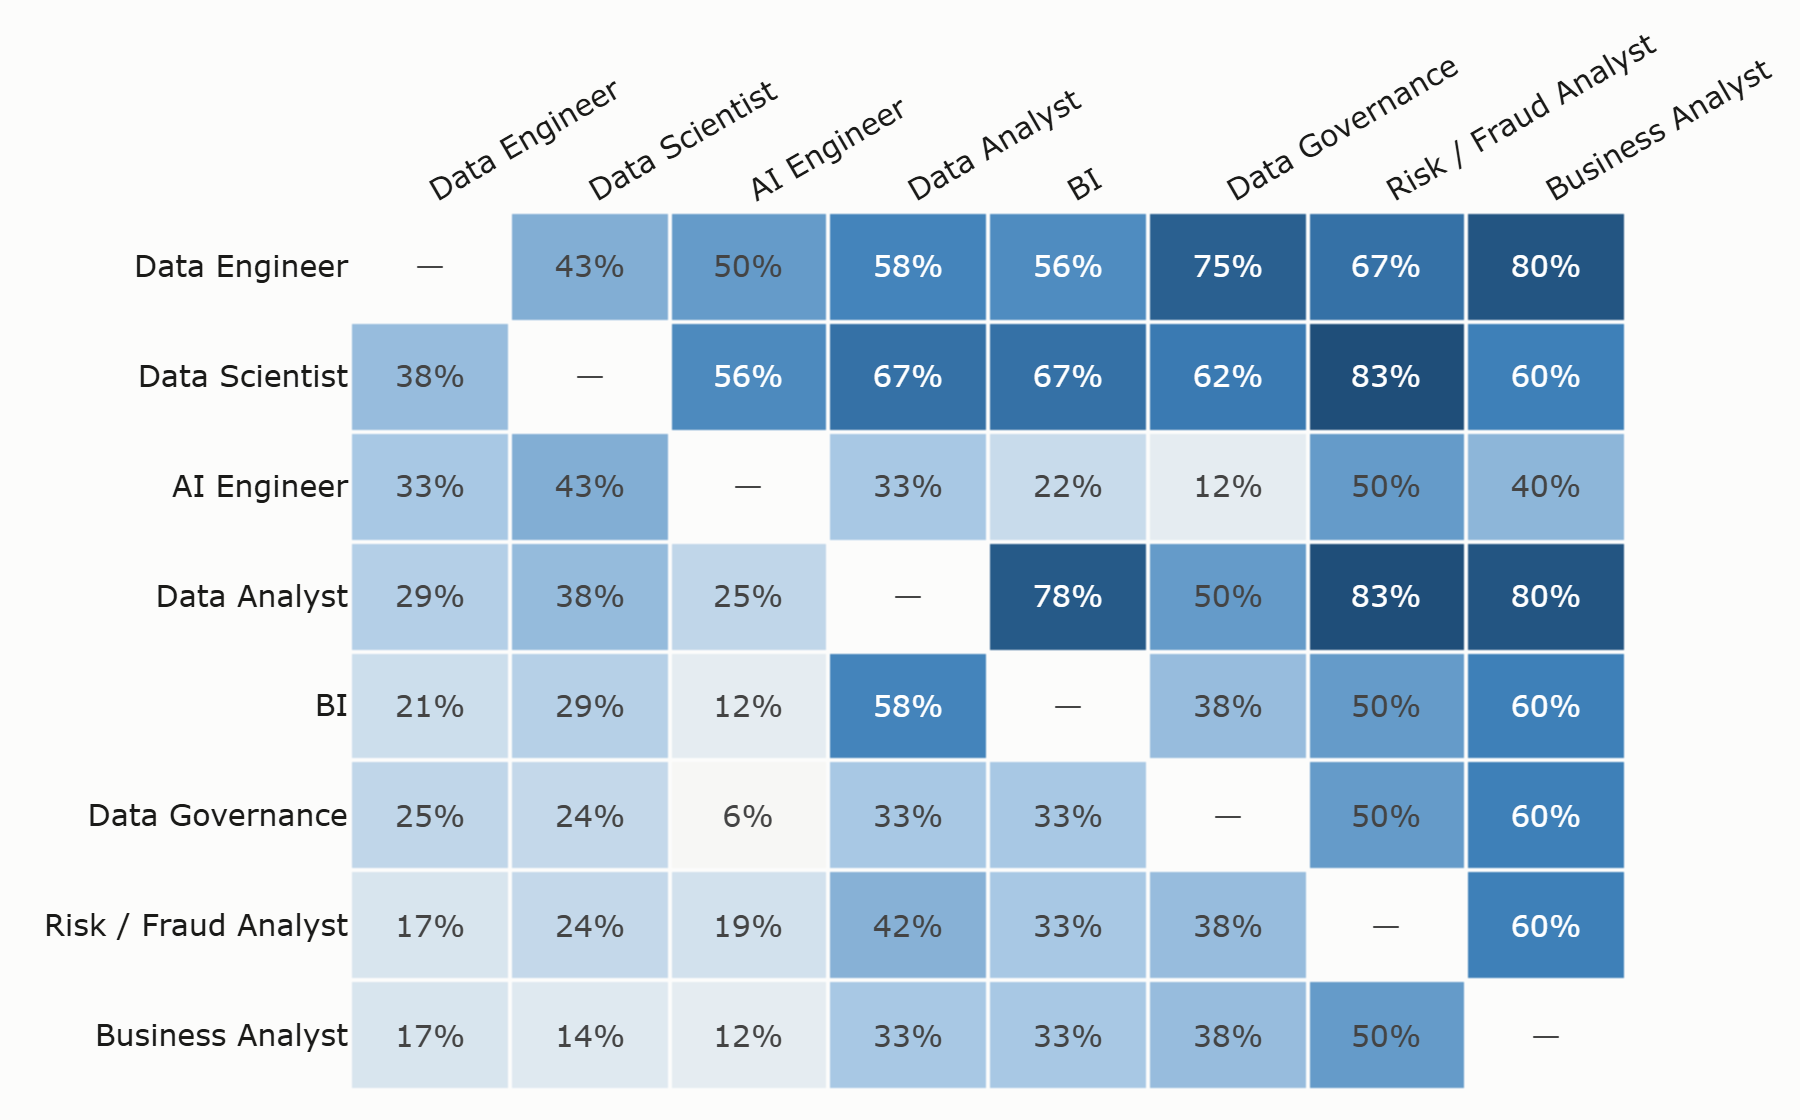
\includegraphics[width=0.78\textwidth]{career_map.png}
\caption{Ma trận chuyển nghề. Ô (hàng $A$, cột $B$) = người làm $A$ đã có sẵn bao nhiêu \% hồ sơ kỹ
năng của $B$.}
\end{figure}

\subsection{Hàng rào tối thiểu để ứng tuyển}

Kỹ năng xuất hiện ở hơn một nửa số tin của nghề đó:

\begin{center}
\small
\begin{tabular}{ll}
\toprule
\textbf{Nghề} & \textbf{Kỹ năng gần như bắt buộc} \\
\midrule
Data Analyst      & Data Analysis, SQL, Reporting, Power BI \\
BI                & Power BI, Reporting, SQL, Data Analysis \\
Data Engineer     & SQL, Python, ETL, Data Management, Data Warehouse, Database \\
AI Engineer       & Python, AI, Machine Learning, LLM, API \\
Data Scientist    & Data Science, Machine Learning, Python, Statistics, SQL \\
Business Analyst  & \textit{chỉ có Business Analysis} \\
\bottomrule
\end{tabular}
\end{center}

\keyfind{Bốn kỹ năng --- đó là hàng rào tối thiểu để ứng tuyển Data Analyst}, không phải mười lăm thứ như
các khoá học thường quảng cáo. Dòng cuối đáng chú ý: Business Analyst chỉ có \emph{đúng một} kỹ năng vượt
ngưỡng, tức nghề này \textbf{không có chuẩn kỹ năng}.

\subsection{Chuyển nghề: thang chỉ đi một chiều}

\begin{center}
\small
\begin{tabular}{lrrr}
\toprule
\textbf{Từ $\downarrow$ \quad Sang $\rightarrow$} & \textbf{Data Analyst} & \textbf{Risk/Fraud} & \textbf{Data Engineer} \\
\midrule
Data Analyst      & ---           & \textbf{83\%} & 29\% \\
Data Engineer     & 58\%          & 67\%          & ---  \\
Business Analyst  & \textbf{33\%} & 50\%          & 17\% \\
\bottomrule
\end{tabular}
\end{center}

\begin{itemize}
\item \keyfind{Thang chỉ đi một chiều.} Data Engineer đã có sẵn 58\% hồ sơ của Data Analyst; chiều ngược
      lại chỉ 29\%. Đi từ kỹ thuật sang phân tích thì dễ, đi ngược lại phải học gần như từ đầu.
      \emph{Nghề đầu tiên chọn quyết định sau này đi được đâu.}
\item \keyfind{Lộ trình rẻ nhất mà ít ai nói tới:} một Data Analyst đã đi được \textbf{83\% đường} sang
      Risk/Fraud Analyst --- và ngân hàng chính là nơi gần như độc chiếm nhánh này (Mục 5.2).
\item \keyfind{Business Analyst: dễ vào, khó ra.} Ai cũng vào được, nhưng người làm BA chỉ giữ 33\% hồ sơ
      của Data Analyst --- hệ quả trực tiếp của việc nghề này không có chuẩn kỹ năng.
\end{itemize}

\subsection{Học theo bó, đừng học lẻ}

Các kỹ năng không xuất hiện rời rạc trong tin tuyển dụng mà đi thành cụm. Ba bó, gần như chỉ giao nhau ở
SQL và Python:

\begin{center}
\small
\begin{tabular}{lll}
\toprule
\textbf{Bó kỹ năng} & \textbf{Gồm} & \textbf{Mở cửa vào} \\
\midrule
Báo cáo    & SQL + Power BI/Tableau + Excel + Reporting     & Data Analyst, BI, Risk/Fraud \\
Hạ tầng    & SQL + Python + ETL + Data Warehouse + Cloud    & Data Engineer \\
AI ứng dụng& Python + Machine Learning + LLM + API + Docker & AI Engineer \\
\bottomrule
\end{tabular}
\end{center}

Học nửa bó thì không mở được cửa nào --- vì hàng rào tối thiểu ở Mục 6.1 đòi \emph{cả} bộ, không đòi từng
món lẻ.

% =====================================================================
\section{Kết luận}

Với 720 tin tuyển dụng thu thập được, thị trường dữ liệu Việt Nam hiện lên khác khá xa hình dung phổ biến:

\begin{enumerate}
\item Đây là thị trường \textbf{phân tích và báo cáo} (Analytics 46,9\%), không phải thị trường
      \emph{xây mô hình} (Data Scientist 4,3\%).
\item \textbf{Không có nghề nào áp đảo} --- bốn nghề lớn nhất chênh nhau trong sai số.
\item Rào cản cho người mới \textbf{không phải số lượng kỹ năng} (Junior 8,2 so với Mid 9,8) mà là kinh
      nghiệm thực chiến.
\item Thứ \emph{phân biệt} một Data Analyst là \textbf{Power BI và Excel}, không phải Python.
\item Chuyển nghề là \textbf{một chiều} --- chọn nghề đầu tiên quan trọng hơn người ta tưởng.
\end{enumerate}

Về mặt phương pháp, phần chúng tôi thấy đáng kể nhất không nằm ở một kỹ thuật phức tạp nào --- toàn bộ
phân tích chỉ là \emph{đếm và so sánh tập hợp} --- mà nằm ở việc dựng được một bộ nhãn nghề \emph{đo được
độ chính xác} (96,7\% qua gán nhãn mù), vì mọi con số phía sau đều phụ thuộc vào nó.

\vspace{4pt}
{\footnotesize
\textbf{Phạm vi diễn giải.} Số liệu mô tả \emph{720 tin thu thập được}, không suy rộng ra toàn thị trường
Việt Nam: mỗi nền tảng được truy vấn với bộ từ khoá khác nhau nên cơ cấu nghề khác nhau đáng kể. Dữ liệu
chỉ có \emph{một lát cắt thời gian}, nên không đưa ra bất kỳ nhận định nào về xu hướng tăng/giảm; và
không có trường lương, nên không có nhận định nào về thu nhập.

\textbf{Tái lập.} Toàn bộ dữ liệu đã gán nhãn được đóng gói trong một cơ sở dữ liệu DuckDB kèm mã nguồn;
mọi bảng số trong báo cáo đều sinh ra từ script và chạy lại được. Số liệu theo lần chạy 03/08/2026.}

\end{document}
